\subsection{Aggiunta di un nuovo software di apprendimento automatico}
Per sostituire il software di apprendimento automatico basterà creare una classe che implementi l'interfaccia \texttt{POSManager} per usare il software di POS-tagging scelto. La nuova classe dovrà realizzare opportunamente i metodi richiesti dall'interfaccia.\\
\vspace*{3em}

\begin{figure}[ht]
	\centering
	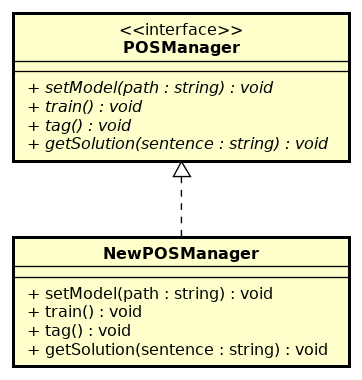
\includegraphics[scale=0.80]{images/newPOS.png}
	\caption{Aggiunta di una vista all'applicazione}
\end{figure}
\newpage

\subsection{Aggiunta di una vista all'applicazione}
Per aggiungere una vista, bisognerà aggiungere anche il relativo presenter. La nuova view dovrà derivare dalla classe astratta \texttt{PageView} e il presenter dovrà derivare da \texttt{PagePresenter}, costruendo nel costruttore il client nel modo che si ritiene più opportuno. Infine, nel costruire la nuova vista bisognerà assegnare il nuovo presenter.\\
\vspace*{3em}

\begin{figure}[ht]
	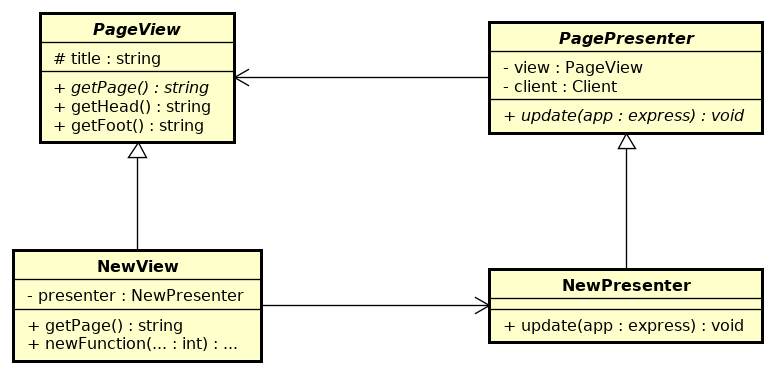
\includegraphics[scale=0.75]{images/newview.png}
	\caption{Aggiunta di una vista all'applicazione}
\end{figure}
\newpage

\subsection{Sostituzione o aggiunta della base informativa}
Per sostituire la base informativa o il modo di interagire con il database, basterà creare delle classi per l'inserimento degli esercizi, delle classi e degli utenti che estendano la classe astratta \texttt{FirebaseManager}.\\
Lo stesso procedimento è valido anche nel caso in cui venga aggiunto un nuovo tipo di informazione nella base di dati.\\
\vspace*{3em}

\begin{figure}[ht]
	\centering
	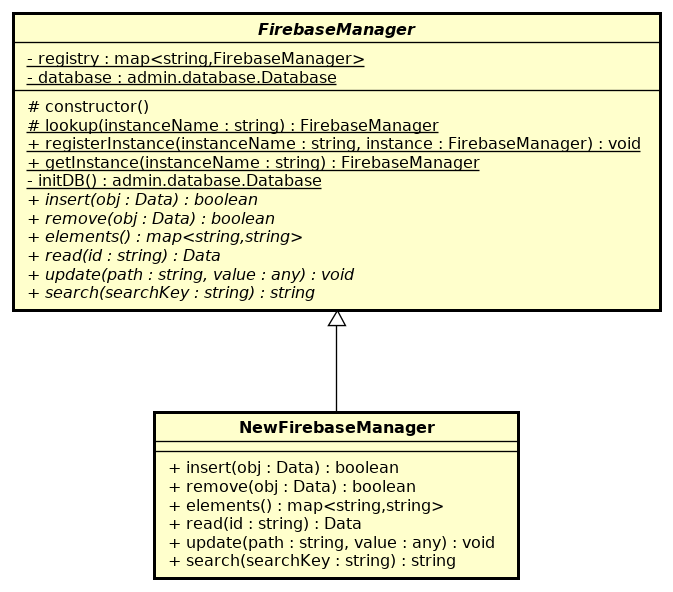
\includegraphics[scale=0.75]{images/newfirebasemanager.png}
	\caption{Aggiunta di una vista all'applicazione}
\end{figure}